\documentclass[12pt]{ctexart}%中文包
\usepackage{graphicx}%图片引用包
\usepackage{amssymb}%特殊符号
\usepackage{amsmath,amsfonts,bm}%矩阵
\usepackage{amsthm}%定理
\usepackage{geometry}%缩放
\usepackage{hyperref}%超链接
\usepackage{framed}%框框
\usepackage{color}%颜色
\usepackage{mathrsfs}%花体
\usepackage{anyfontsize}
\usepackage{indentfirst}%缩进
\usepackage{extsizes}%size
\usepackage{newtxtext,newtxmath}%times风格字体
\usepackage{mdframed}%边栏

\surroundwithmdframed[
  linecolor=gray,
  topline=false,
  bottomline=false,
  rightline=false,
  linewidth=4pt,
  innerleftmargin=10pt,
  innerrightmargin=10pt,
  innertopmargin=0pt,
  innerbottommargin=10pt
]{theorem}
\surroundwithmdframed[
    linecolor=black,
    leftline=false,
    rightline=false,
    linewidth=0.5pt,
    innerleftmargin=10pt,
    innerrightmargin=10pt,
    innertopmargin=0pt,
    innerbottommargin=10pt
]{note}

\newtheorem{theorem}{Law}
\newtheorem{note}{Note}



\geometry{a4paper,scale=0.85}
\hypersetup
    {
        hypertex=true,
        colorlinks=true,
        linkcolor=blue,
        anchorcolor=blue,
        citecolor=blue
    }


\title{Introduction to Laser\\激光绪论}

\author{Jerry Ling} 

\date{\today}
 
\begin{document}
\maketitle
主要参考书: \textit{Laser Electronics} by Joseph. 授课老师陶镇生是物理系教授,他的研究方向集中于超快激光和光物质作用。本课程的前置物理知识主要是电动力学和基础量子力学,前置数学知识主要是波动方程和偏微分方程组。
\section*{何为激光}
\textbf{Laser},本意为[Light Amplication by Stimulated Radiation]。实际上的核心部件由谐振腔和增益介质构成。为了对激光的特性和其原理有概念性的认识,我们将从其一般特点出发作为绪论的开始。
\subsection*{一般特点}
\par 在空间传播方面,激光有极强的\textbf{指向性}。此外,激光谐振腔能够产生特定模式的光束,令发射光具有良好的数学性质。注意,光束的边缘必然是衰减、而非锐利的,否则其横向动量将导致强烈的衍射。作为参考,若激光器的孔径为$D=1cm$,那么高斯光束的发散角约在$\lambda/D$量级,即约10$\mu$ rad。而半导体激光器由于本身薄层发射,原始发散角较大(空间频率分布更宽)。尽管如此,总是有办法通过透镜将相干光调制为准直光。
\par 在能量方面,一般的激光器能产生$\textup{mW}$量级的功率。最早的Ruby激光器能达到$\textup{kW}$量级,而超快激光器能达到$\textup{GW}$级的峰值功率。
\par \textbf{相干性}是激光器最突出的特点之一。空间相干:同一时刻两点的光的步调一致性或相位差稳定性。时间相干:同一路径上不同时间的光的步调一致性或相位差稳定性。而激光器产生的电磁波具有高度可控的相干性。
\par Note: 波长换算至光子能量:
\begin{equation}
    E = \frac{1240}{\lambda (nm)}\textup{eV}
\end{equation}
\subsection*{频率特性}
\par 连续波激光器可产生高度单一频率的波,而短脉冲/超快激光则发生波包产生的频谱展宽。后者需要使用其他频段的电磁波在中心外的地方发生相消,即\textbf{锁模技术(Mode-locking)}的原理。
\begin{equation}
    \Delta t \approx \frac{1}{2 \Delta \omega}
\end{equation}
注意,上式在各频率相位相同时取等号,也就是在频域相位一致时取\textbf{Transform Limit}。直观理解为在相位完全一致处有最大叠加、而在周围相位快速散开而在时域强度衰减。
\par 当然,激光还可能在各种方面偏离正弦波。除了波段造成的展宽,反射造成的\textbf{衰减(absorption loss)}将造成洛伦兹展宽;介质(如声子)造成的\textbf{相位突变(decoherence)}则造成高斯或更复杂的展宽。
\begin{note}[comparation of band width]
    \par 不妨考虑一个最简单的辐射体——黑体辐射。令黑体内部有若干简单两能级气体被一盏白织灯激发,并测量一个小的出口处的频谱。这些气体被激发后仍能够在黑体内不断反射,因而其被激发的时间和运行到出口的时间是完全紊乱的。i.e.黑体辐射给出非相干的输出。
    \begin{equation}
        I(\nu, T)=\frac{2h\nu^3}{c^2}\frac{1}{e^{h\nu/kT}-1}
    \end{equation}
注意上述Plank通过热分布所导出的辐射密度须要内部气体的能级差覆盖所有波段。而日常常见的白织灯也是一种非相干光源,其频谱宽度~10 $\textup{GHz}$。作为对比,激光器的带宽可做到$<\textup{MHz}$。
\end{note}
\par 一般而言,介质不止有一种发射频段。所以我们需要\textbf{谐振腔(cavity)}放大某一频段的光。本质上cavity利用了驻波的原理,具有若干\textbf{模式(modes)}。令其长度为L:
\begin{equation}
    L = \frac{n \lambda_n}{2} \ \ \ \ \
    f_n = n \frac{c}{2L}
\end{equation}
因而,谐振腔可以具有一定的频率选择能力。其允许的频率构成梳状的条谱,从而调整激光器的频率。作为参考,1000nm的近红外光在1m的谐振腔中需要$10^6$级的模式。而注意实际情况中,由于衰减和损失,允许频率是有展宽的。
\section*{谐振器}
\textbf{谐振器(resonator)}是物理中常见的一种结构。从秋千到RC电路都属于谐振结构,能够在特定频率下产生共振。为了避免衰减,resonator需要一种驱动力来维持其本征频率的振荡。这种补偿需要coherent,即与振荡步调一致,好比摇秋千时需要适时地推一把才能维持周期运动。在激光器中,这种对反射损失的补偿通过\textbf{增益(gain)}来实现。
\par 一般而言,增益介质可以令某一频率的谐振模式重新变回\textbf{连续波(cw)}模式,从而达到极窄的带宽。要注意,没有增益是无法实现窄线宽的。而放大的基本原理基于\textbf{受激辐射(stimulated emission)}。注意其同自发辐射相比,属于触发事件而非指数随机过程,因而是与激发光同相的。而这其中最重要的条件是\textbf{非平衡(population inversion)}态的介质。关于介质的能级条件,将在后续笔记中讨论。
\par 下面我们从简单的统计力学考察一个两能级介质:
\begin{equation}
    \frac{N_1}{N_2}=exp\{-\frac{e_2-e_1}{kT}\}
\end{equation}
显然在平衡态下N2的布局数总是小于等于N1(即使温度趋于无穷大)。即使在使用光激发电子向上越迁,由于受激的过程系数一致,一旦N2布局数更高,其立刻更快地会越迁回到N1。i.e.二能级系统不可能达到反转的状态。
\par 因而,我们必须选取至少具有三个能级的粒子作为介质。这样,只要把电子给泵到高能级上,令其长时间地逗留在\textbf{亚稳态},就能造成亚稳态和基态之间的粒子数反转。实践上可用转动、振动、电子等多种能级来实现。
\begin{figure}[t] 
    \centering
    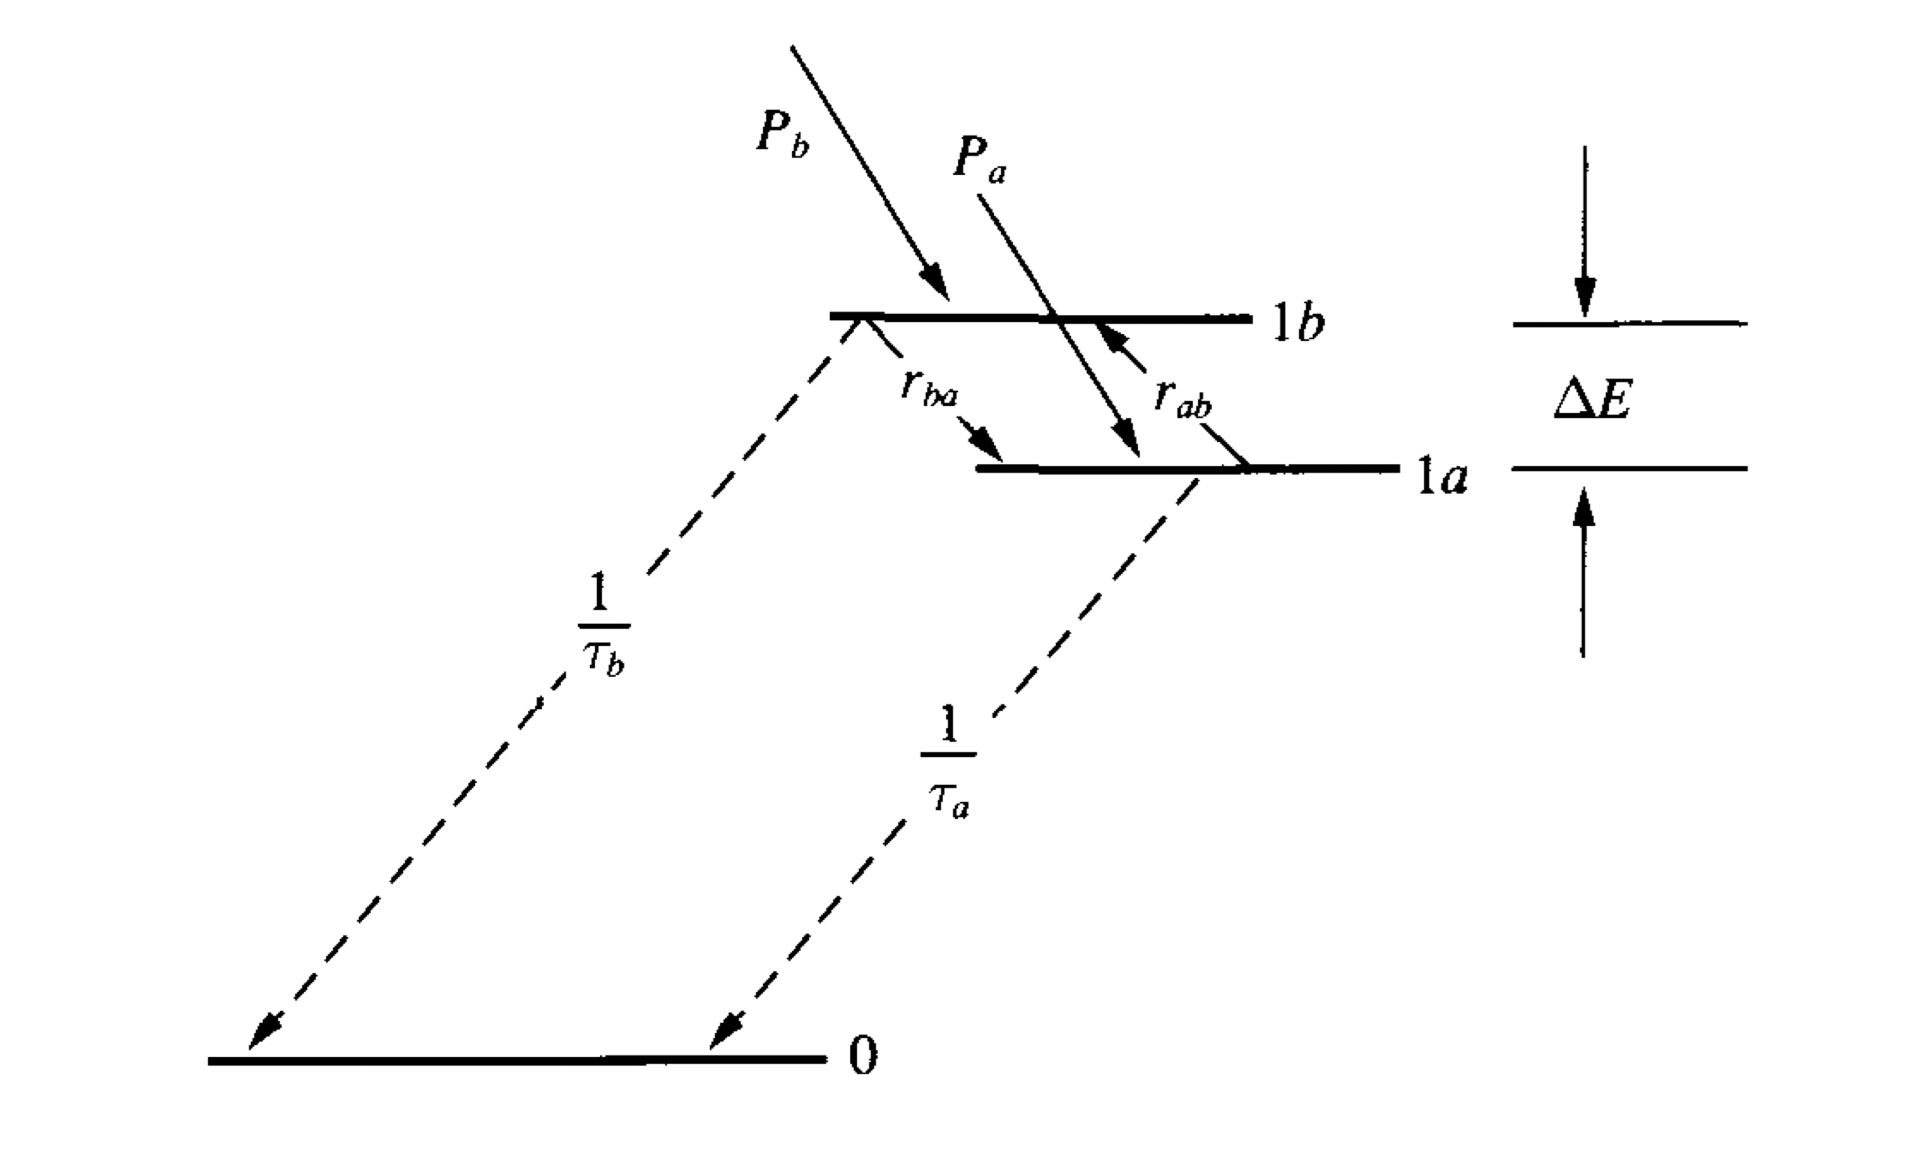
\includegraphics[width=0.6\textwidth]{energy_level.png}
    \caption{A three level system}
    \label{three level system}
\end{figure}
\par 最后,需要注意谐振腔的模式之间只有$\textup{MHz}$的间隔(frequency comb),而放大系统通常要覆盖若干根线。尽管如此,我们可以调整其放大曲线的\textbf{临界点},使其只有一个频率线在无数次传播时被放大:$ Gain * Loss\geq 1$当然,调节L,即谐振腔大小也会导致频率的移动,有时候温度的升高也会导致这种微动。用\textbf{标准具(Etalon)}或棱镜对也可以调节光程或调节反射情况,从而达到选择频率的效果。


\end{document}